\begin{appendices}

\chapter{Appendices}
\label{ch:appendices}

\section{Appendix A - Deployment Roles \& Users}
\label{appendix:roles_users}

Mind Map representing the identified user roles of the Department of Computing Science in red to the left and the identified users in blue to the right.

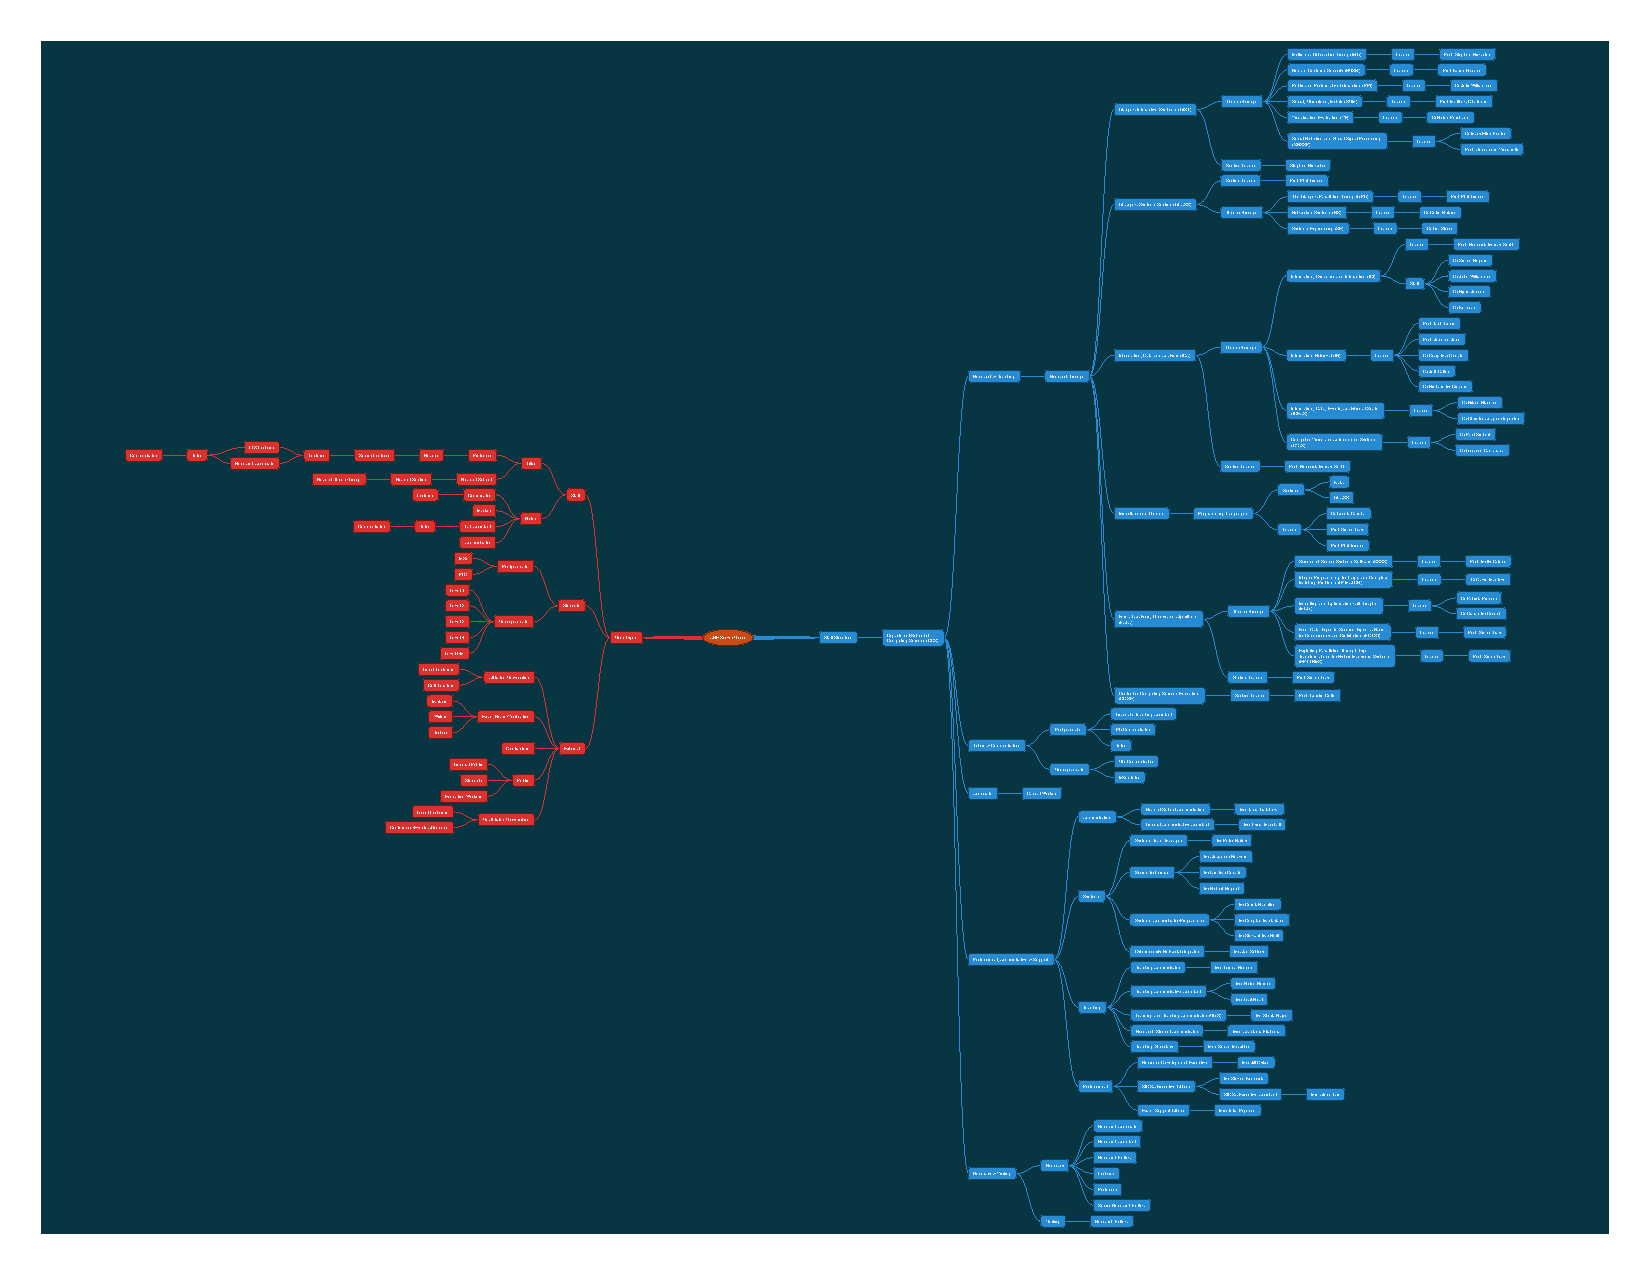
\includegraphics[width=\linewidth]{appendices/mind_maps/ABE_Users_slides_Oct26.pdf}

\section{Appendix B - Enrolment Diagram for Staff User}
\label{appendix:enrolment_diagram}

\begin{figure}
    \centering
    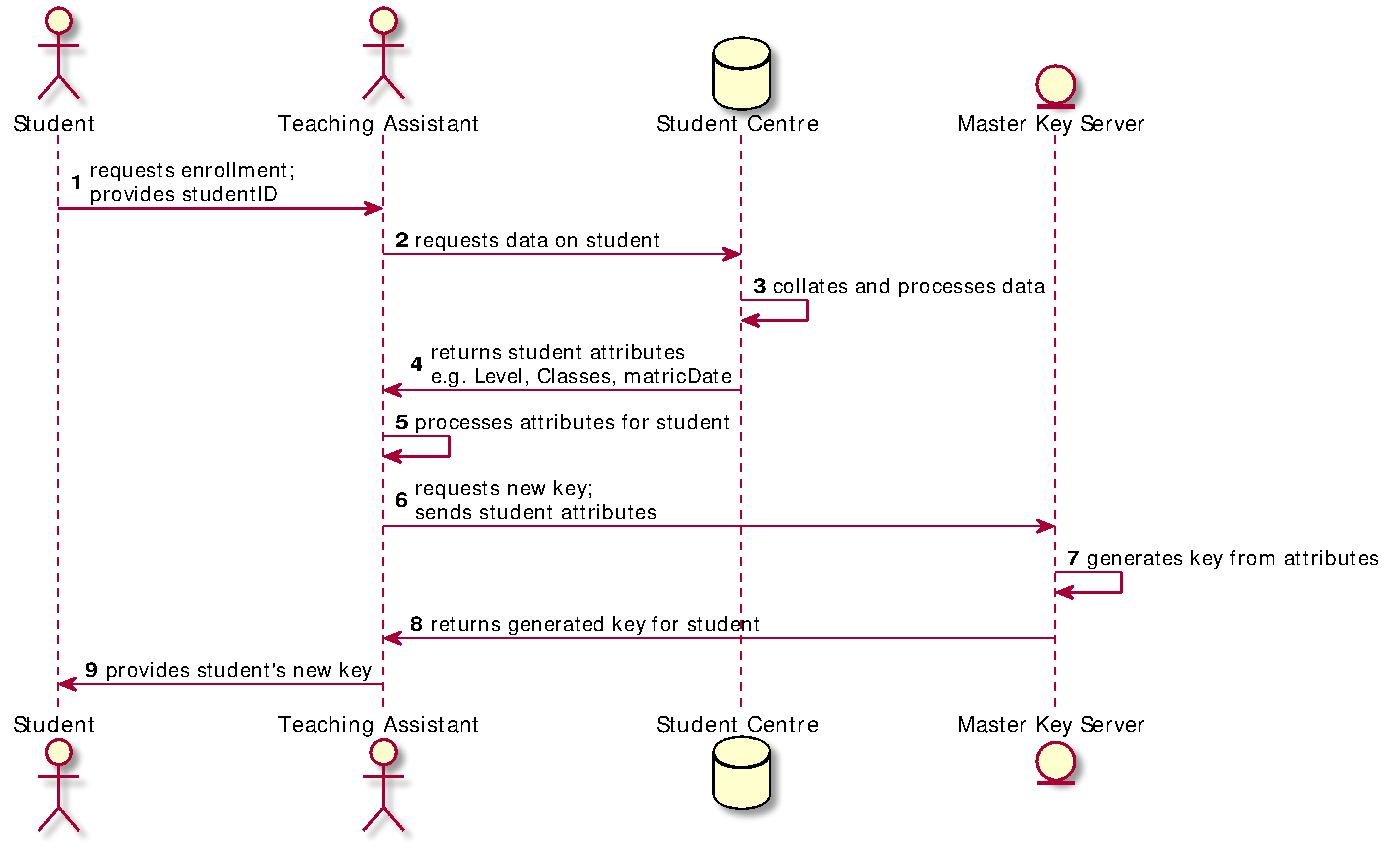
\includegraphics[width=\linewidth,keepaspectratio]{appendices/diagrams/flow_of_info/enrollment_stu_sequence.pdf}

    \caption{A sequence diagram demonstrating the enrolment process for a student. The student can be seen requesting a user key \#1 (and providing their student ID) from the DCS Teaching Assitant, whom verifies the student's identity and then retrieves their details \#2 from the Student Centre (or MyCampus) system. The Teaching Assistant then processes the returned attributes \#5 for the Master Key Server, and then requests a new key \#6 by providing the student's attributes. The Master Key Server can be seen processing \#7 and then returning the newly generated key \#8 to the Teaching Assistant, whom finally provides the key to the student.}

\end{figure}

\end{appendices}
